\subsection{Гистограммы}
\label{subsec:result_hist}
\begin{itemize}
	\item{Нормальное распределение}
	\begin{figure}[H]
		\centering{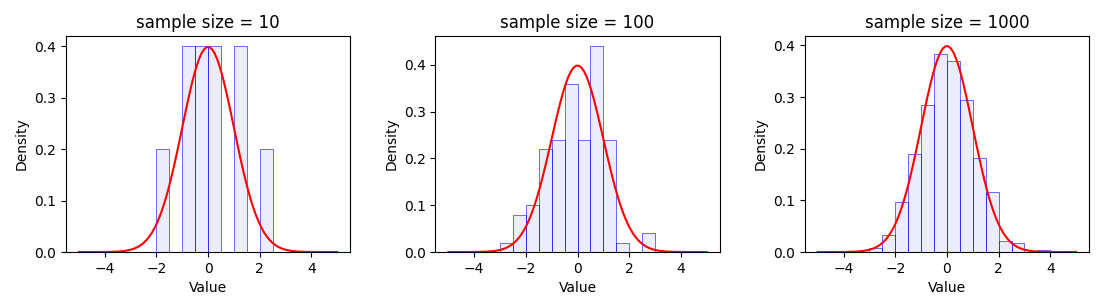
\includegraphics[scale=0.6]{part_hist/figures/normal}}
		\caption{Гистограмма и плотность вероятности для нормального распределения [N = 10, 100, 1000]}
		\label{fig:hist_normal}
	\end{figure}
	
	\item{Распределение Коши}
	\begin{figure}[H]
		\centering{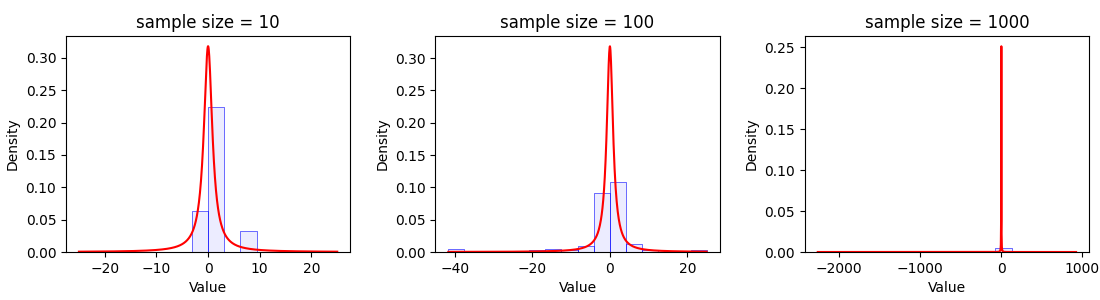
\includegraphics[scale=0.6]{part_hist/figures/cauchy}}
		\caption{Гистограмма и плотность вероятности для распределения Коши [N = 10, 100, 1000]}
		\label{fig:hist_cauchy}
	\end{figure}
		
	\item{Распределение Лапласа}
	\begin{figure}[H]
		\centering{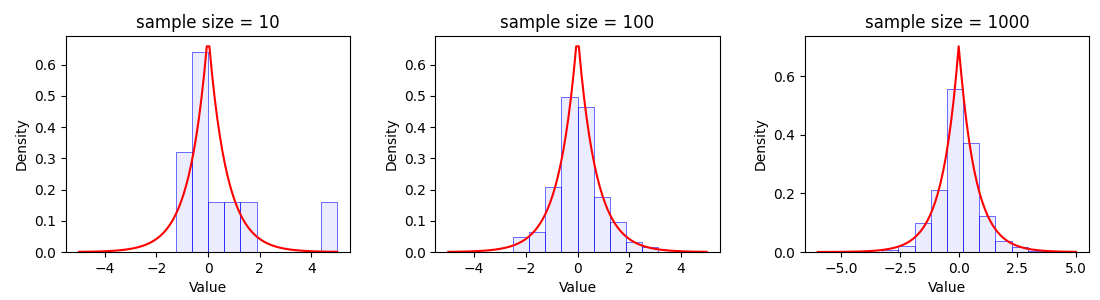
\includegraphics[scale=0.6]{part_hist/figures/laplace}}
		\caption{Гистограмма и плотность вероятности для распределения Лапласа [N = 10, 100, 1000]}
		\label{fig:hist_laplace}
	\end{figure}
		
	\item{Распределение Пуассона}
	\begin{figure}[H]
		\centering{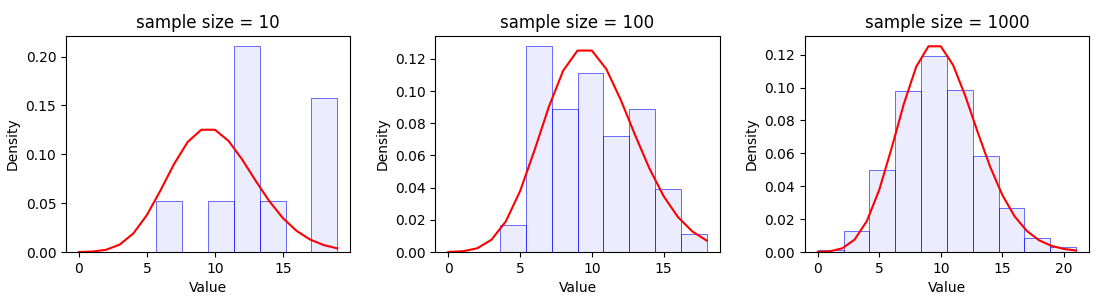
\includegraphics[scale=0.6]{part_hist/figures/poisson}}
		\caption{Гистограмма и плотность вероятности для распределения Пуассона [N = 10, 100, 1000]}
		\label{fig:hist_poisson}
	\end{figure}
	
	\item{Равномерное распределение}
	\begin{figure}[H]
		\centering{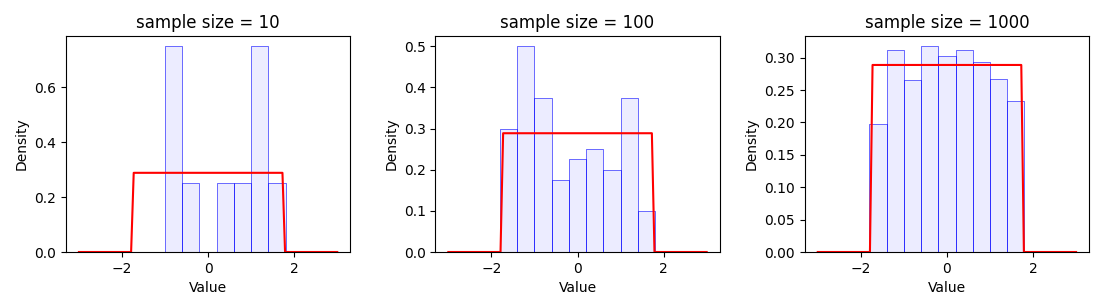
\includegraphics[scale=0.6]{part_hist/figures/uniform}}
		\caption{Гистограмма и плотность вероятности для равномерного распределения [N = 10, 100, 1000]}
		\label{fig:hist_uniform}
	\end{figure}

\end{itemize}